\chapter{Convolutional Nerual Networks}
\label{chap:chap4}

\section{Tổng quan}
\textit{Convolutional Neural Network }(CNNs – Mạng nơ-ron tích chập) là một trong những mô hình Deep Learning tiên tiến giúp cho chúng ta xây dựng được những hệ thống thông minh với độ chính xác cao. Trong khóa luận này, tôi sẽ trình bày về  Convolution (tích chập) cũng như xây dựng mô hình CNNs cho bài toán nhận dạng chữ viết tay trong tiếng Nhật (Image Classification).\par
Lấy cảm hứng từ xử lý ảnh nên đầu vào và các lớp của CNNs có dạng như một bức ảnh chứ không có dạng vector như Neural Networks thông thường. Cụ thể, một bức ảnh sau khi số hoá có dạng \textit{width $\times$ height $\times$ depth} (width: số lượng điểm ảnh trên chiều rộng, height: số lượng điểm ảnh trên chiều cao, depth: số lượng kênh chẳng hạn như RGB có 3 kênh đại diện cho mức độ của 3 màu Đỏ, Lục, Lam). Mô hình được mô tả ở Hình \ref{fig:conv}

\begin{center}
\begin{figure}[H]
\label{fig:conv}
\begin{center}
\subfloat[mạng nơron thông thường]
  {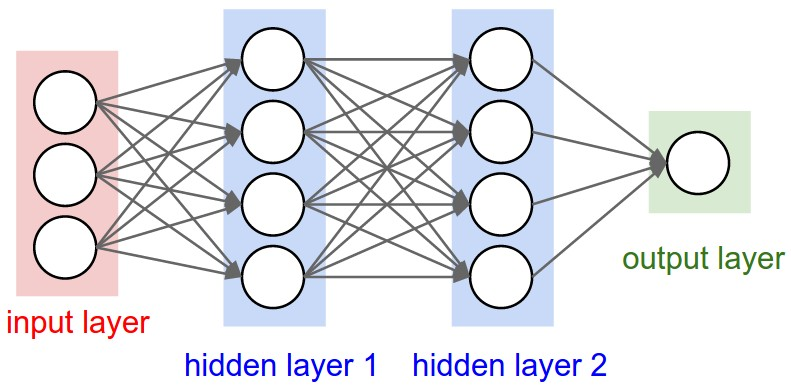
\includegraphics[width=.3\linewidth]{chap4/image/architectureNNs}}
\subfloat[mạng nơron tích chập]
  {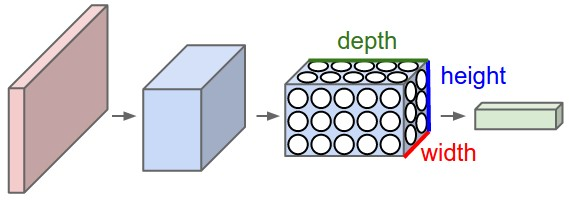
\includegraphics[width=.3\linewidth]{chap4/image/architectureCNN}}
\caption{Kiến trúc hai mạng}
\end{center}

\end{figure}
\end{center}

Một mạng CNNs đơn giản có ba lớp chính: lớp tích chập (\textit{convolutional layer}), lớp giảm số chiều (\textit{pooling layer}), lớp fully-connected. Các lớp convolutional và lớp pooling được xếp xen kẽ nhau Hình \ref{fig:convNetArch}.
\begin{center}
\begin{figure}[H]
	\begin{center}
		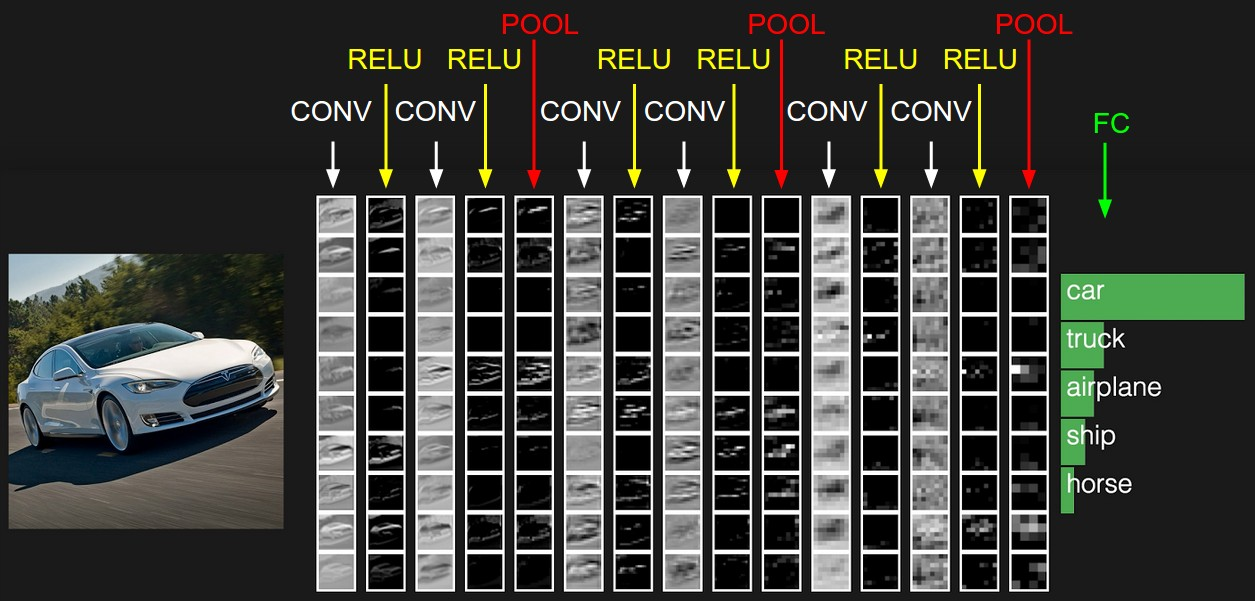
\includegraphics[scale=0.2]{chap4/image/convnet.jpeg}
	\end{center}
	\caption{ví dụ về kiến trúc của ConvNets}
	
\label{fig:convNetArch}
\end{figure}
\end{center}
\section{Bộ lọc và cửa sổ trượt}
Trước khi đi đến chi tiết các lớp, chúng ta cần hiểu \textit{bộ lọc (filter)} là gì, \textit{cửa sổ trượt (sliding window)} là gì.
\subsection{Bộ lọc - filter}
Như tôi đã trình bày ở phần trên, kích thước của đầu vào đã thay đổi thành dạng khối. Vì thế kích thước của trọng số cũng được thay đổi thành dạng khối để phù hợp với hình dạng của đầu vào và nó còn được gọi là \textit{filter} hoặc \textit{kennel}.  Ví dụ như Hình \ref{fig:filter}, ma trận I là ma trận đầu vào, ma trận K là filter và ma trận I*K là ma trận kết quả (được trình bày ở phần sau).
\begin{center}
\begin{figure}[htp]
	\begin{center}
		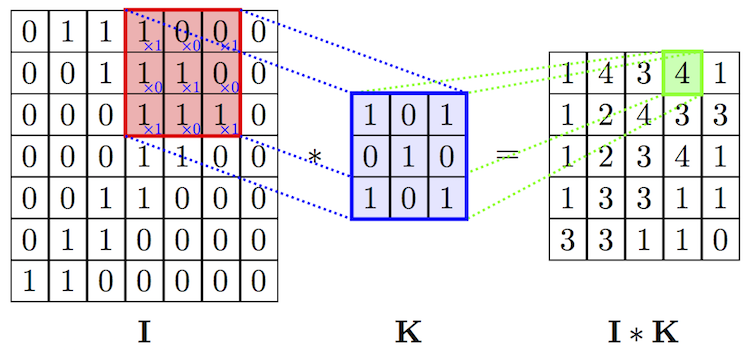
\includegraphics[scale=1.2]{chap4/image/minhHoaTichChap.png}
	\end{center}
	\caption{Bộ lọc - filter}
	\label{fig:filter}
\end{figure}
\end{center}
Kích thước của các filter thường là $d\times3\times3$, $d\times5\times5$, $d\times7\times7$  hoặc $d\times11\times11$, trong đó $d$ là chiều sâu của filter, hai tham số tiếp theo thể hiện chiều rộng và chiều cao của filter. Chú ý rằng chiều sâu của filter luôn luôn bằng chiều sâu của đầu vào.
\subsection{Cửa sổ trượt - sliding window}
\textit{Cửa sổ trượt (sliding window)} là ta chọn một "cửa sổ" có kích thước nhỏ hơn kích thước đầu vào và trượt cửa sổ đó trên đầu vào theo chiều ngang và chiều dọc. Các bước trượt là khoảng cách mà ta dịch chuyển filter trên đầu vào và đó gọi là \textit{stride}, ký hiệu là $s$. Ví dụ như Hình \ref{fig:slidingwindow}, ta có đầu vào kích thước là $5\times5$, cửa sổ có kích thước là $3\times3$ và tại mỗi bước trượt cửa sổ dịch chuyển đi một đơn vị, do đó stride bằng 1.
\begin{center}
\begin{figure}[htp]
	\begin{center}
		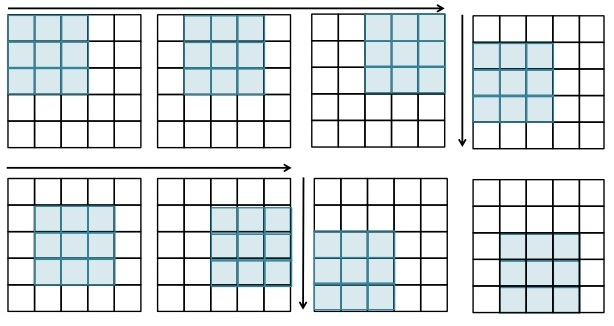
\includegraphics[scale=1]{chap4/image/slidingwindow.jpg}
	\end{center}
	\caption{Sliding window}
	\label{fig:slidingwindow}
\end{figure}
\end{center}

\section{Lớp tích chập - Convolutional layer}
Convolution layer là khối cốt lõi, cơ bản của ConvNets, lớp này chủ yếu nặng về việc tính toán. Lớp này chính là nơi thể hiện tư tưởng ban đầu của mạng nơron tích chập. Thay vì kết nối toàn bộ điểm ảnh, lớp này sẽ sử dụng bộ lọc (\textit{filter}) áp vào một vùng trong ảnh và tiến hành tính tích chập giữa bộ filter và giá trị điểm ảnh trong vùng cục bộ đó,  vùng này ta gọi là \textit{receptive filter}. Sau đó ta dùng sliding window để trượt filter và tiến hành tích chập tại mỗi vùng ta trượt đến. Tôi sẽ trình bày chi tiết thông qua Hình  \ref{fig:tinhtoanConv}.

\begin{figure}[htp]

\subfloat[\label{fig:slide1_1}]
  {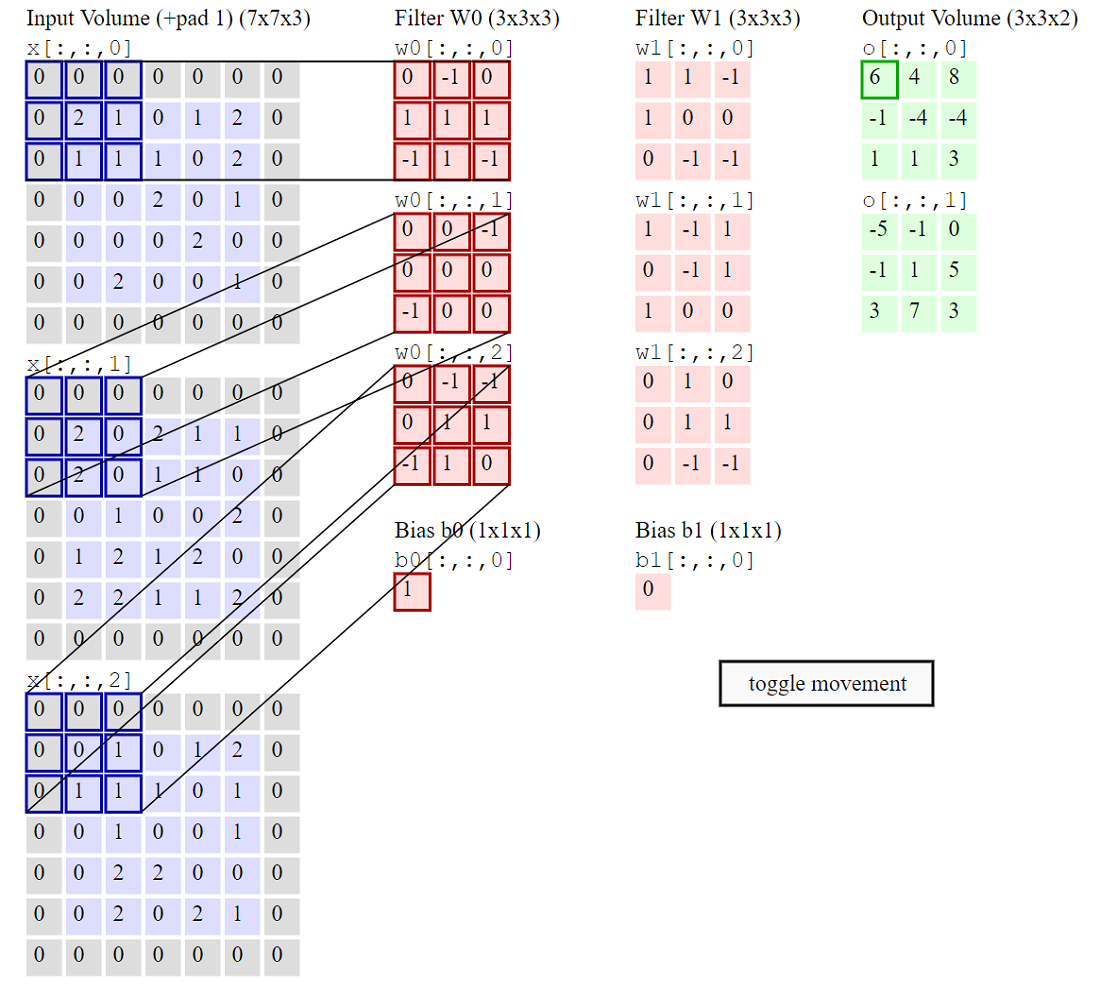
\includegraphics[width=.3\linewidth]{chap4/image/slide1_1.png}}\hfill
\subfloat[\label{fig:slide1_2}]
  {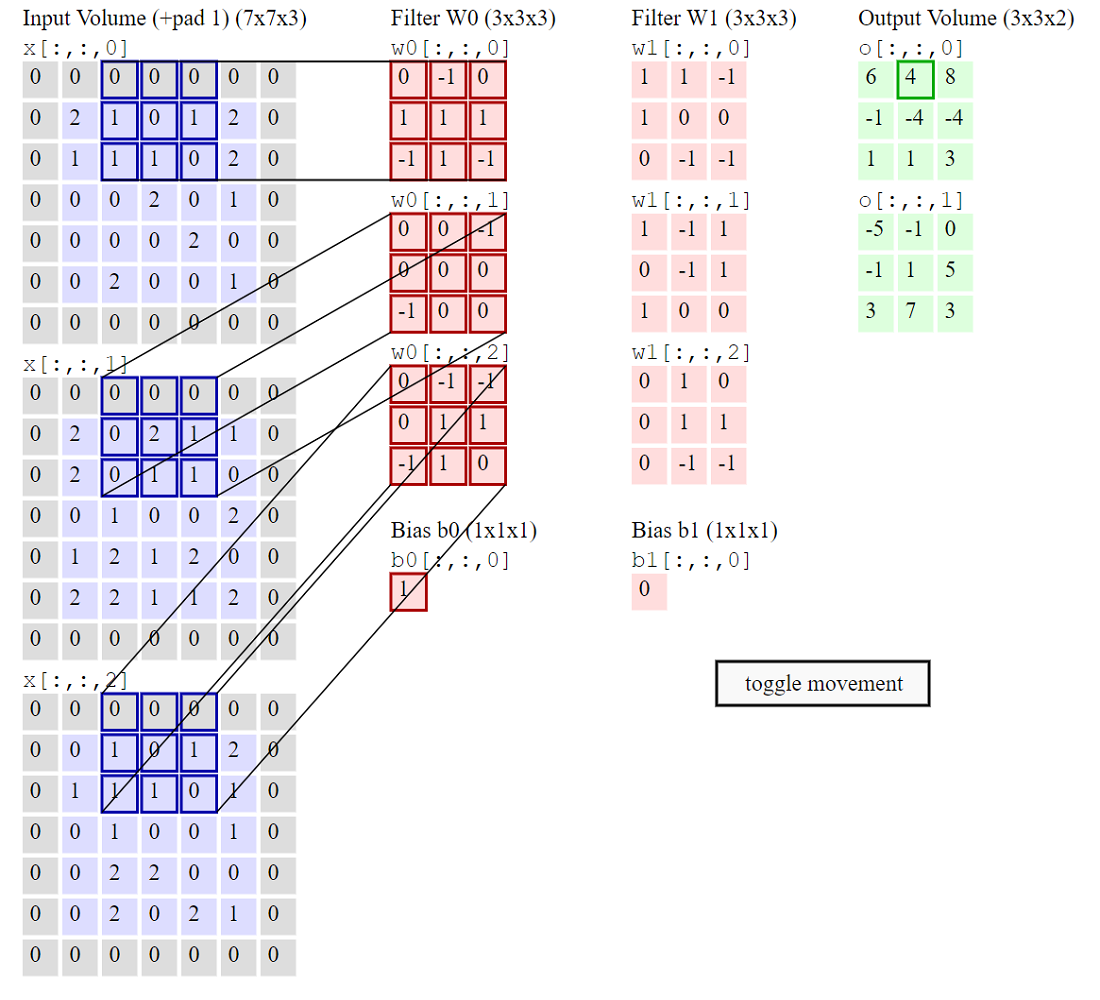
\includegraphics[width=.3\linewidth]{chap4/image/slide1_2.png}}\hfill
\subfloat[\label{fig:slide1_3}]
  {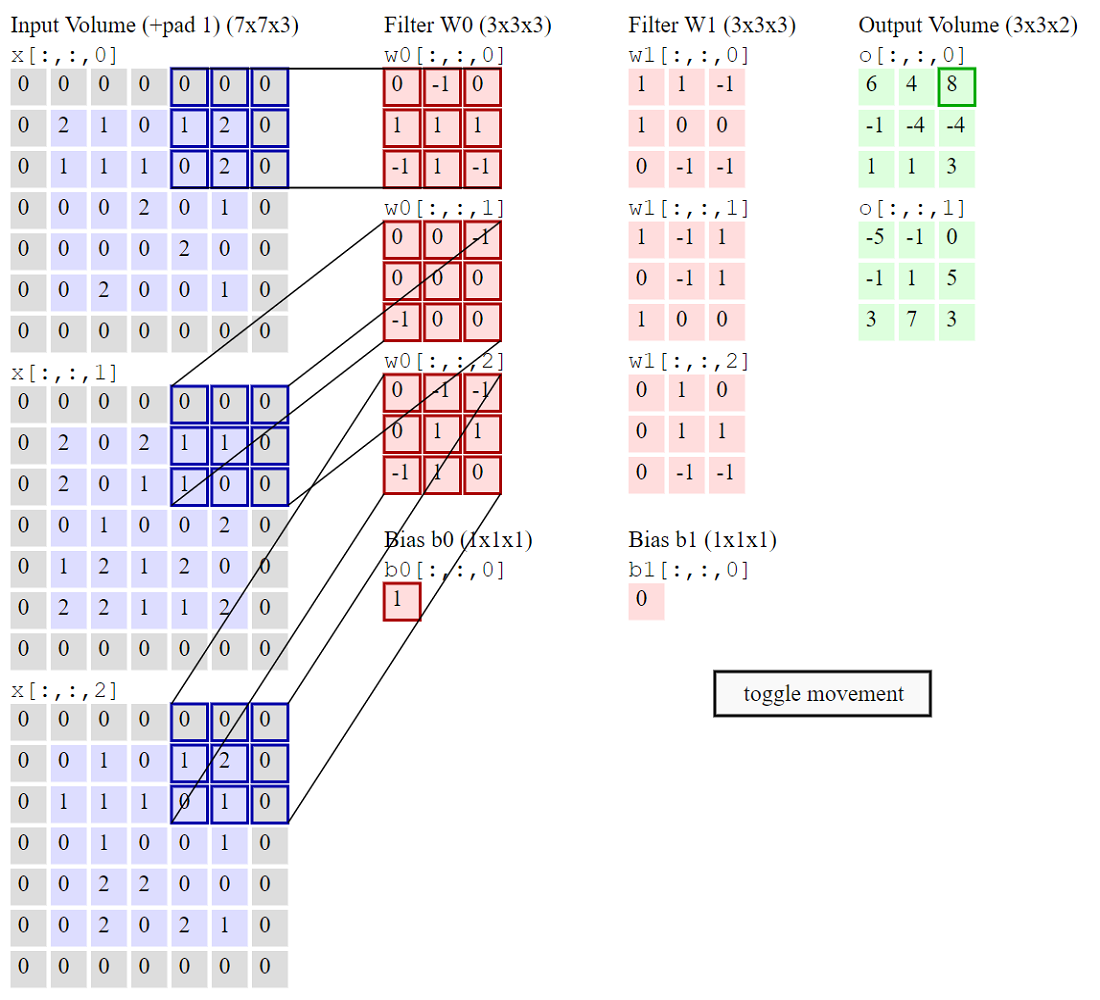
\includegraphics[width=.3\linewidth]{chap4/image/slide1_3.png}}\\
\subfloat[\label{fig:slide2_1}]
  {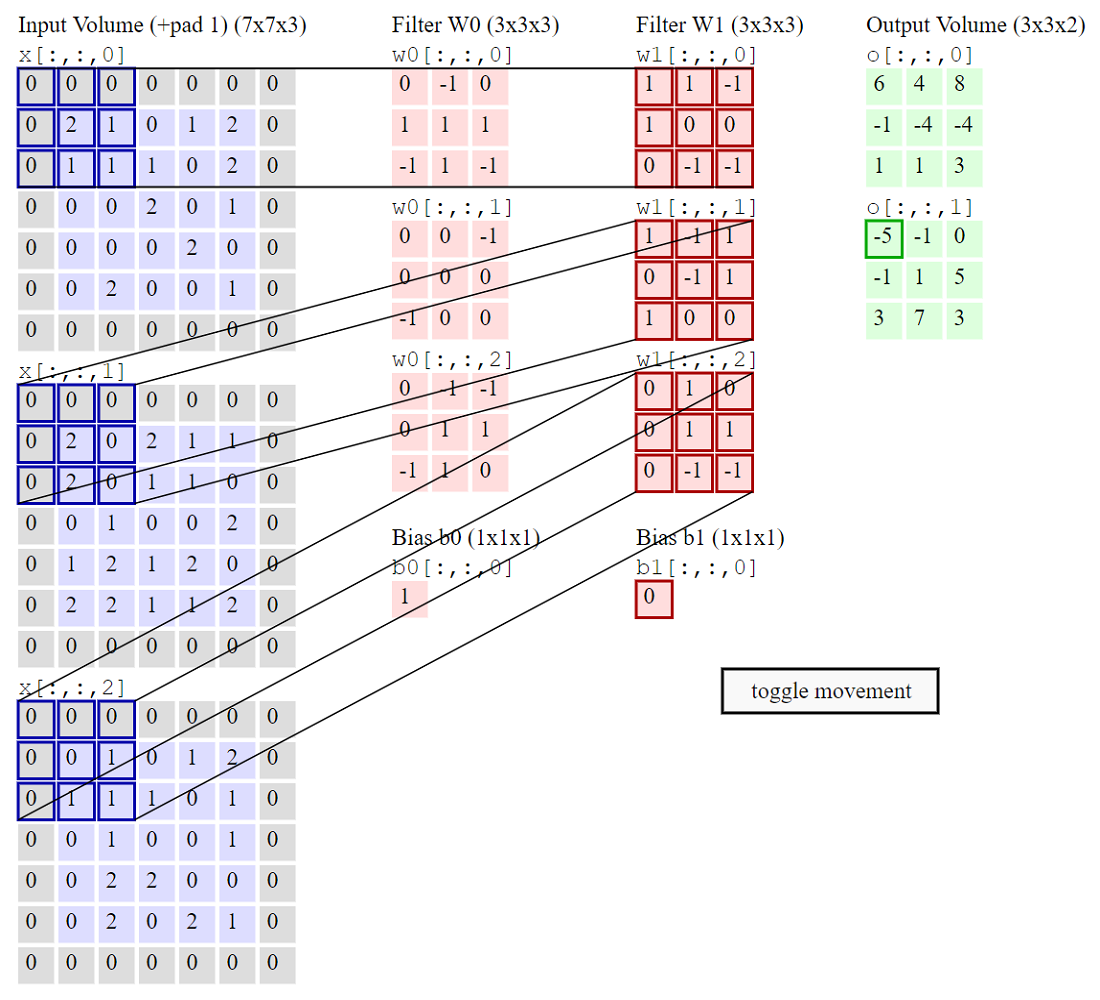
\includegraphics[width=.3\linewidth]{chap4/image/slide2_1.png}}\hfill
\subfloat[\label{fig:slide2_2}]
  {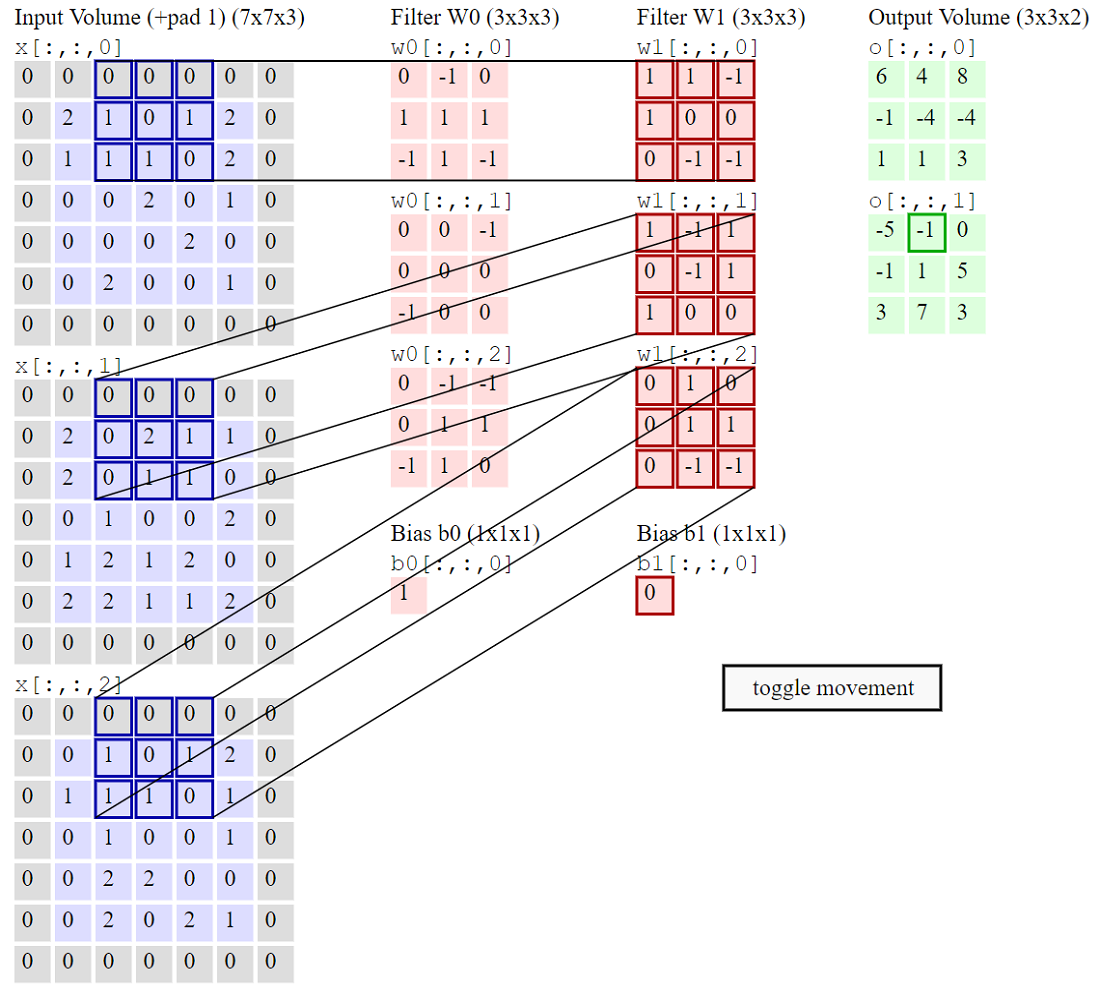
\includegraphics[width=.3\linewidth]{chap4/image/slide2_2.png}}\hfill
\subfloat[\label{fig:slide2_3}]
  {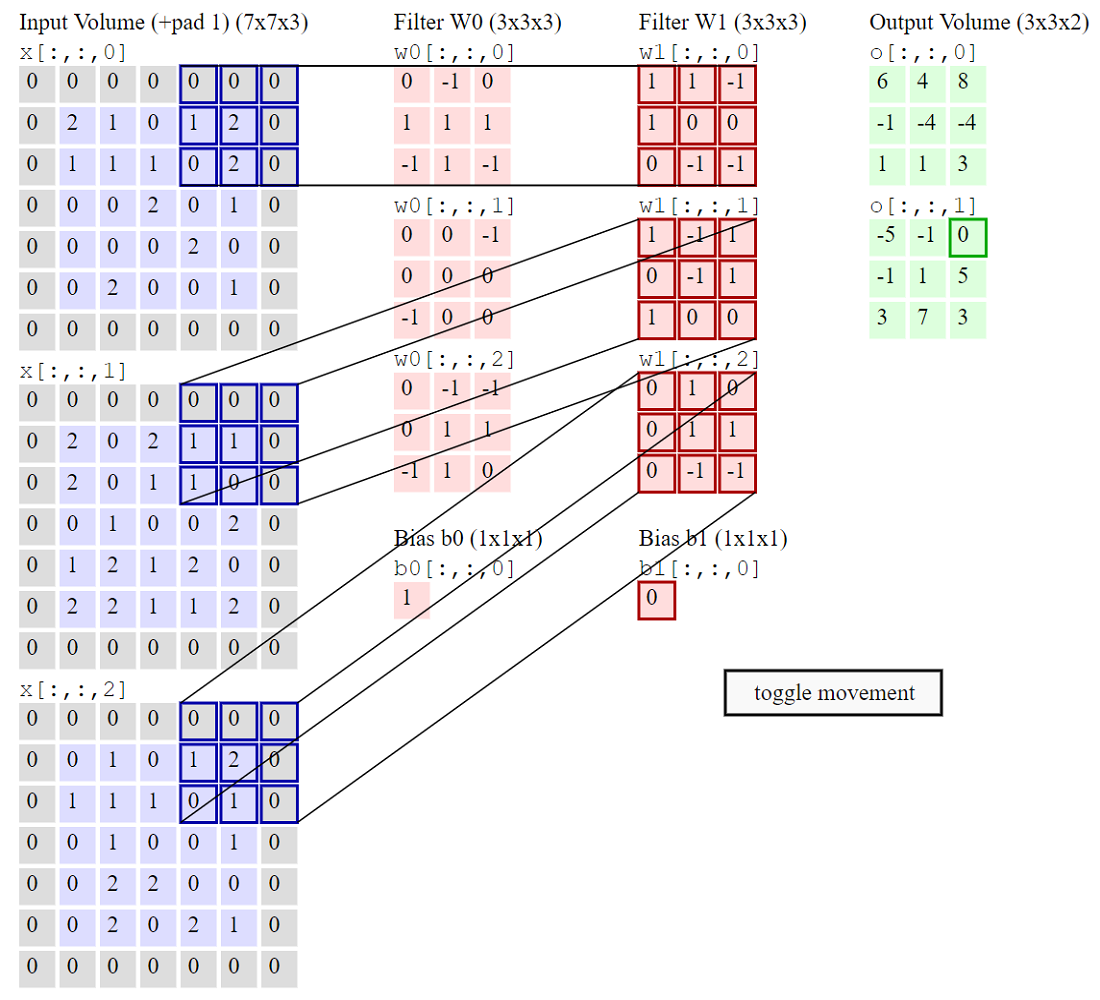
\includegraphics[width=.3\linewidth]{chap4/image/slide2_3.png}}
\caption{Tính toán trong lớp tích chập}
\label{fig:tinhtoanConv}
\end{figure}

Theo Hình \ref{fig:tinhtoanConv} ta có kích thước đầu vào là $7 \times 7\times 3$, stride bằng 2, kích thước filter là  $2\times 3\times 3 \times 3$ với 2 là số \textit{channel} (số chanel sẽ là chiều sâu output chúng ta mong muốn). Tại Hình \ref{fig:slide1_1} ta  thực hiện phép tính... tương ứng giữa receptive filter, $filter ~W0$ tại tất cả các độ sâu, kết quả được cộng thêm $bias$ rồi lưu vào ma trận output vị trí đầu tiên của đầu ra. Sau đó ta thực hiện cách tính toán trên kết hợp sliding window với stride bằng 2 và filter là $filter W0$, kết quả ta thu được là ma trận output thứ nhất, các Hình \ref{fig:slide1_1}, \ref{fig:slide1_2}, \ref{fig:slide1_3} mô tả giai đoạn này. Và tương tự như trên ta thực hiện với $filter ~W1$ theo Hình \ref{fig:slide2_1}, \ref{fig:slide2_2}, \ref{fig:slide2_3} ta thu được kết quả là ma trận thứ hai tại output. Như vậy nếu ta có càng nhiều channel thì chiều sâu output của chúng ta càng lớn. \par

Nếu như đầu ta chỉ tính trên kích thước đầu vào thì với filter $3\times 3$ và stride bằng 2 thì ta chỉ trượt được hai lần và đến hàng, cột thứ 5 của đầu vào còn giá trị tại hàng, cột thứ 6, 7 sẽ không được tính. Vì thế chúng ta thêm vào ma trận đầu vào các hàng và cột đối xứng với giá trị bằng 0 để không ảnh hưởng đến đầu vào mà khi đó ta sẽ quét được hết các giá trị của đầu vào. Cách này được gọi là \textit{zero padding}. Như ở ví dụ trên ta thấy đầu vào được bao quanh bởi các số 0 và kích thước tăng thành $8 \times 8$, đó là ta áp dụng zero padding với p=1.\par
Ta có công thức để tính toán kích thước đầu ra như sau:
\begin{itemize}
	\item Kích thước đầu vào \textbf{$W_1$} x \textbf{$H_1$} x \textbf{$D_1$} (rộng x cao x sâu)
	\item Kích thước của filter \textbf{$F$}
	\item Số channel \textbf{$K$}
	\item Tốc độ trượt \textbf{$S$}
	\item Giá trị của zero-padding \textbf{$P$}
	\item Kích thước đầu ra \textbf{$W_2$} x \textbf{$H_2$} x \textbf{$D_2$}:
	\begin{itemize}
		\item[+]  \textbf{$W_2 = (W_1 - F+ 2P)/S +1$}
		\item[+] \textbf{$H_2 = (H_1 - F+ 2P)/S +1$}
		\item[+] \textbf{$D_2 = K$}
	\end{itemize}	 
\end{itemize}	

\begin{center}
\begin{figure}[htp]
	\begin{center}
		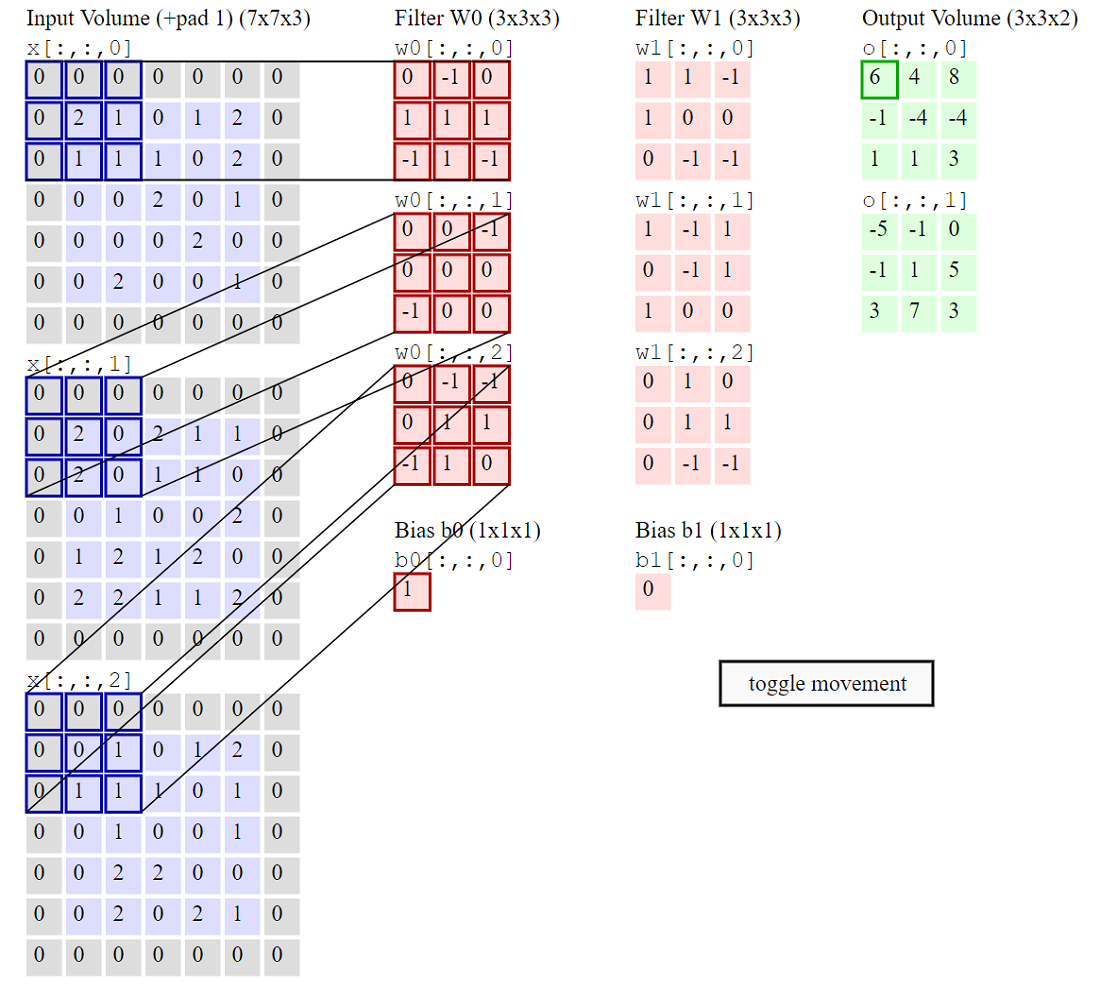
\includegraphics[scale=0.2]{chap4/image/slide1_1.png}
	\end{center}
	\caption{Ví dụ về tính toán kích thước đầu ra}
	\label{fig:minhhoatichchap2}
\end{figure}
\end{center}
Giả sử ta có thông số như hình \ref{fig:minhhoatichchap2} với kích thước đầo vào là $7\times7\times3$ tương đương $W=H=7,~ D_1=3$;stride $S=3$; kích thước filter là $2\times 3\times 3 \times 3$ hay $F=3$ và số channel $K=2$. Theo công thức ta tính được $(W_1 - F+ 2P)/S$ không phải là số nguyên do đó ta cần thêm padding để giá trị này là số nguyên. Ta chọn $P=1$ vì $(7-3+2\times 1)/3 +1$ là số nguyên. Như vậy ta tính được kích thước đầu ra sẽ là $3\times3\times2$. \par
Một phần quan trọng của layer này đó là hàm activation, hàm này được tính với đầu vào là kết quả sau khi thực hiện tích chập. Và ReLU thường được chọn là hàm activation do tính đơn giản của nó. Nhiệm vụ của nó là chuyển toàn bộ giá trị âm trong kết quả sau khi tích chập thành 0. Ý nghĩa của cách cài đặt này chính là tạo nên tính phi tuyến cho mô hình. 
\section{Lớp giảm số chiều -  pooling layer}
\textit{Lớp giảm số chiều (pooling layer)} trong mạng CNNs thực hiện công việc loại bỏ bớt những thông tin không cần thiết sau khi thực hiện tích chập và được chèn giữa các lớp convolutional với nhau hoặc sau một tập lớp convolutional. Nó có vai trò giảm kích thước dữ liệu. Với một bức ảnh kích thước lớn qua nhiều lớp pooling sẽ được thu nhỏ lại tuy nhiên vẫn giữ được những đặc trưng cần cho việc nhận dạng (thông qua cách lấy mẫu). Việc giảm kích thước dữ liệu sẽ làm giảm lượng tham số, tăng hiệu quả tính toán và góp phần kiểm soát hiện tượng quá khớp (overfitting). Tuy nhiên nếu lạm dụng loại layer này cũng có thể khiến data đi qua bị mất dữ liệu.\par
\textbf{Cách thức hoạt động}: Pooling layer sử dụng sliding window và tại mỗi cửa sổ trượt trên đầu vào chỉ có một giá trị được xem là giá trị đại diện cho thông tin ảnh tại vùng đó (giá trị mẫu) được giữ lại và đó gọi là tiến hành lấy mẫu (\textit{subsampling}). Các phương thức lấy phổ biến trong pooling layer là \textit{Max pooling} (lấy giá trị lớn nhất), \textit{Min pooling} (lấy giá trị nhỏ nhất) và \textit{Average Pooling} (lấy giá trị trung bình). Hình \ref{fig:pool} mô tả tiến hành lấy mẫu bằng max pooling.\par

\begin{center}
\begin{figure}[H]
	\begin{center}
		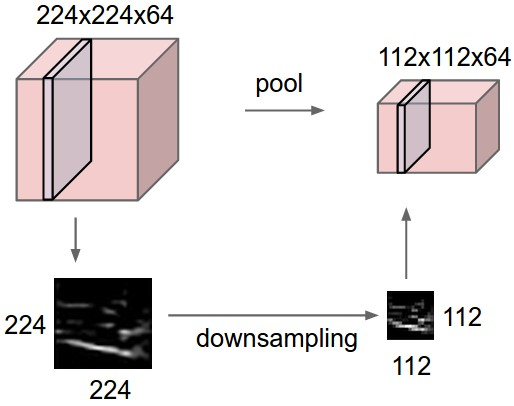
\includegraphics[scale=0.5]{chap4/image/poolEx.jpeg}
	\end{center}
	\caption{Minh họa giảm số chiều}
	\label{fig:pool}
\end{figure}
\end{center}

Ví dụ ta có ma trận đầu vào $4\times 4$  như hình \ref{fig:poolExample}, với kích thước cửa sổ áp dụng cho slidiing window là $2\times 2$ và stride = 2, điều này tương đương với việc ta chia ma trận đầu vào thành 4 ma trận con với kích thước là $2\times2$.  Phương thức ta áp dụng tại đây là max pooling, do đó tại mỗi cửa sổ khi ta áp vào đầu vào thì ta sẽ chọn giá trị lớn nhất làm đại diện cho cửa sổ đó và ta thu được kết quả là ma trận $2\times2$ bên tay phải.\par
\begin{center}
\begin{figure}[htp]
	\begin{center}
		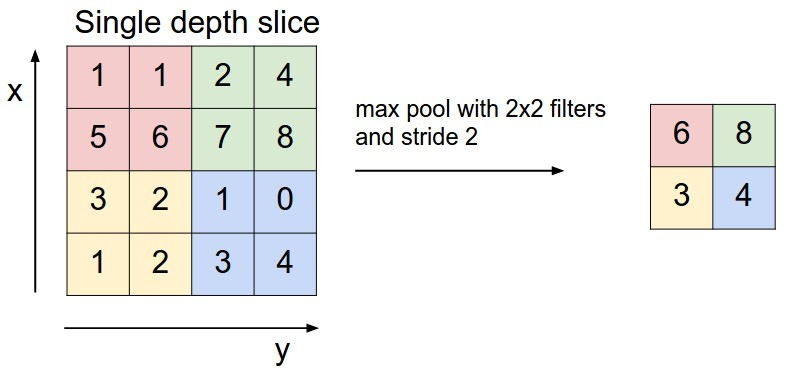
\includegraphics[scale=0.5]{chap4/image/maxpoolEx.jpeg}
	\end{center}
	\caption{Max pooling}
	\label{fig:poolExample}
\end{figure}
\end{center}
Ta rút ra được công thức tính kích thước đầu ra cho lớp này như sau:
\begin{itemize}
	\item Kích thước đầu vào \textbf{$W_1$} x \textbf{$H_1$} x \textbf{$D_1$} (rộng x cao x sâu),
	\item Kích thước cửa sổ \textbf{$F$},	
	\item Tốc độ trượt \textbf{$S$}
	\item Kích thước đầu ra \textbf{$W_2$} x \textbf{$H_2$} x \textbf{$D_2$}:
	\begin{itemize}
		\item  \textbf{$W_2 = (W_1 - F)/S +1$}
		\item  \textbf{$H_2 = (H_1 - F)/S +1$}
		\item \textbf{$D_2 = D_1$}
	\end{itemize}	 
\end{itemize}
Chú ý rằng chúng ta không thường xuyên sử dụng $zero~padding$ cho lớp này.
\section{Lớp Fully-Connected (Fully-Connected layer)}
Sau khi ảnh được xử lý và trích xuất đặc trưng bằng các lớp convolutional, pooling thì ta sẽ làm phẳng (flatten) output cuối cùng của giai đoạn trước đó và áp dụng mạng nơron truyền thẳng với input là dữ liệu ta vừa làm phẳng. Hay nói cách khác Fully-Connected chính là một mạng nơron được gắn vào phần cuối của CNNs với input là đầu ra của các lớp trước đó. Nó đóng vai trò như một mô hình phân lớp và tiến hành dựa trên dữ liệu đã được xử lý ở các lớp trước đó.
\section{Tổng kết}
Dưới đây là một mô hình mạng CNNs kết hợp giữa các layer với nhau với cấu trúc như sau: Conv $\to$ Max-pool $\to$ Conv (giữ nguyên kích thước) $\to$ Max-pool $\to$ Conv (giữ nguyên kích thước) $\to$ Conv (giữ nguyên kích thước) $\to$ Conv (giữ nguyên kích thước) $\to$ Max-pool $\to$ Flatten $\to$ FC . Kích thước các lớp được thể hiện tại Hình \ref{fig:CNN}.
\begin{center}
\begin{figure}[H]
	\begin{center}
		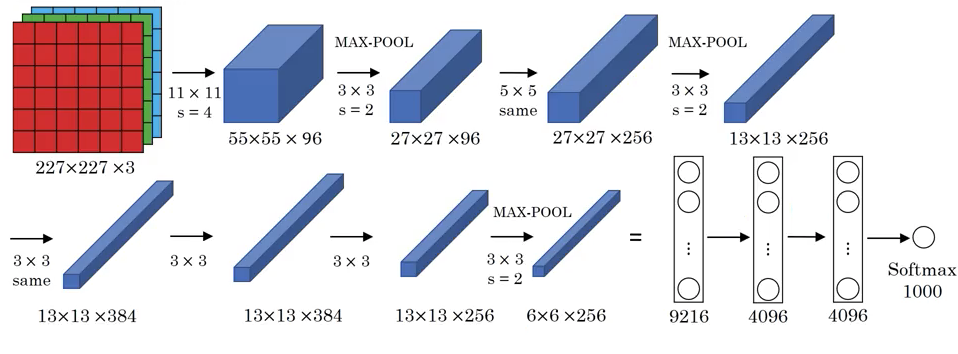
\includegraphics[scale=0.5]{chap4/image/CNN.png}
	\end{center}
	\caption{Ví dụ cấu trúc mạng CNNs}
	\label{fig:CNN}
\end{figure}
\end{center}
